\documentclass[12pt]{article}

\usepackage{amsthm}
    \newtheorem{definition}{Definition}

%\usepackage[default]{raleway}
\usepackage{setspace}
    \doublespacing%
\usepackage[margin=1in, includefoot, footskip=30pt]{geometry}

\usepackage{caption}
\usepackage{color}
\usepackage{booktabs}
\usepackage{graphicx}
\usepackage{hyperref}
\usepackage{wrapfig}

\newlength{\imgwidth}
\newlength{\logoheight}
\setlength{\imgwidth}{.75\paperwidth}
\setlength{\logoheight}{.125\paperheight}

\title{Novel methods for the analysis of NHS patient-episode data}
\author{%
    Henry Wilde\\
    \small{Supervised by: Dr Jonathan Gillard \& Dr Vincent Knight}
}


\begin{document}
\titlepage{%
    \maketitle
    \vfill%
    \makebox[\linewidth]{%
        \includegraphics[height=\logoheight]{../img/cu_logo.png}%
        \hfill%
        
\includegraphics[height=\logoheight]{../img/cthb_logo.jpg}
    }
    \thispagestyle{empty}
    \pagebreak%
}

\setcounter{page}{1}
\tableofcontents%
\pagebreak%

In this section we will conduct a summative and exploratory analysis of the data
provided by the Cwm Taf University Health Board. The focus will be on the
distributions of, and relationships between, our non-trivial cost components
and a selection of other clinical attributes such as length of stay and number
of diagnoses. As we will see in the ensuing analysis, the bulk of this data
corresponds to short-stay and relatively low-cost spells of treatment. Following
this, we will endeavour to construct a framework for the analysis of slices
within the data which provide another dimension to our analysis through
comparison and contrast. However, before any such analysis begins, it is
important to understand the structure of data we are dealing with and how it has
been prepared.

\subsection{Data structure}\label{subsec:structure}

The data is comprised of approximately two and a half million episode-level
records for patients from across Wales that are being treated in the Prince
Charles and Royal Glamorgan hospitals. An episode is defined to be any
continuous period of care provided by the same consultant in the same place. For
instance, if a patient is admitted to a general medical ward for diagnosis and
testing, and then is referred to a specialist consultant in oncology their first
episode would end and be recorded, and a second episode of care would begin on
the oncology ward. Each of these episodes would correspond to a row in the
dataset. If the patient was then discharged, they would have completed a spell
with two episodes. In this analysis we will avoid looking at episode-level
statistics in favour of a patient's spell-level statistics. Since the
introduction of the `payment by results' system for financial flows, it has been
seen that focusing on the more granular episode statistics can lead to the
amount of resource or `activity' consumed by a hospital to treat that patient
being overestimated~\cite{BMJ2004}.

Each episode is recorded as a row of roughly 250 attributes or columns,
including:

\begin{itemize}
    \item Personal identifiers such as identification numbers, age, registered
        GP practice, as well as spell admission and discharge dates;
    \item Other clinical quantities such as the number of diagnoses and
        procedures conducted in that episode, admission and discharge methods,
        and length of stay;
    \item A number of cost components which include the costs coming from
        various departments within the hospital, ward and overhead costs, and
        the cost of administration;
    \item Diagnosis (HRG, ICD10) and procedure (OPCS4) indicators, as well as
        Charlson index scores for a selection of common diagnoses.
\end{itemize}

Of the attributes listed here, we will focus on the cost components and other
clinical variables, paying particular attention to those attributes which are
considered to be linked to overall contribution to the cost of care. Other than
the cost components themselves, those attributes are: true length of stay,
maximum number of diagnoses and total number of procedures in a spell, and the
number of spells associated with any given patient.

\subsection{Cleaning the data}\label{subsec:formatting}

As with many \-- if not all \-- machine learning and knowledge discovery
applications, a substantial amount of preprocessing and formatting was required
to make the data consistent and suitable for our purposes. This process included
the removal of some superfluous columns which added no real information to the
dataset, and a number of rows that had been corrupted by some external storage
software during data collection. In addition to this, we reformatted some
columns whose entries were intended to be used as datetime objects later on.

\graphicspath{{./img/overview/}}
As was discussed in Section~\ref{subsec:structure}, the vast majority of our
attributes will not be considered at this stage of our analysis so we can focus
on how the cost of care is distributed and seen in the data. The exclusion of
these attributes does not, however, imply that they are not of interest. 

\subsection{Distributions and summative
statistics}\label{subsec:distributions_statistics}
\graphicspath{{./img/general/}}

When we look at the distributions of our subset of attributes on the whole
dataset we see that the data is skewed towards low-cost, short-stay, and
otherwise low-impact patients with long, heavy tails, as seen in
Figures~\ref{fig:netcost_kde}~\--~\ref{fig:no_spells_hist}. We can then take
advantage of the other attributes to identify slices of the dataset which are of
interest by literature review, clustering, or otherwise.

In the following plots, and subsequently, when we refer to `spell-level'
quantities, we mean that each of our cost components and the number of
procedures are summed over all episodes in any given spell, the number of
diagnoses at the spell level is considered as the maximal number of diagnoses in
a spell, and the length of stay is unique to the spell not the episode. The
decision to take the maximal number of diagnoses as opposed to the total number
of diagnoses is justified since, (a.) we want to minimise the effect of counting
the same diagnosis more than once at the spell level, and (b.) the severity of a
patient's condition is often compared against their Charlson comorbidity
index~(CCI), which a weighted summation of their individual
severities~\cite{Thygesen2011}. As such, by taking the maximum number of
diagnoses we hope to capture the most severe a patient's condition becomes
during a spell as this is often indicative of how aggressive the patient's
treatments are, and thus likely more expensive due to additional drug or ward
costs, for instance.

\begin{figure}[h]
    \centering
    \begin{minipage}{.495\textwidth}
        \includegraphics[width=\linewidth]{netcost_kde/main.pdf}
        \captionof{figure}{Estimated probability density for the net cost of a
        spell, clipped at \pounds12,500.}\label{fig:netcost_kde}
    \end{minipage}\hfill%
    \begin{minipage}{.495\textwidth}
        \includegraphics[width=\linewidth]{los_hist/main.pdf}
        \captionof{figure}{Histogram for the total length of a spell, clipped at
        21 days.}\label{fig:los_hist}
    \end{minipage}
\end{figure}

\begin{figure}[h]
    \centering
    \begin{minipage}{.495\textwidth}
        \includegraphics[width=\linewidth]{no_diag_hist/main.pdf}
        \captionof{figure}{Histogram for the number of diagnoses in an
        episode.}\label{fig:no_diag_hist}
    \end{minipage}\hfill%
    \begin{minipage}{.495\textwidth}
        \includegraphics[width=\linewidth]{no_proc_hist/main.pdf}
        \captionof{figure}{Histogram for the number of procedures in an
        episode.}\label{fig:no_proc_hist}
    \end{minipage}
\end{figure}

\begin{figure}[h]
    \centering
    \begin{minipage}{.495\textwidth}
        \includegraphics[width=\linewidth]{no_spells_hist/main.pdf}
        \captionof{figure}{Histogram for the number of spells associated with a
        patient.}\label{fig:no_spells_hist}
    \end{minipage}\hfill%
    \begin{minipage}{.495\textwidth}
        \includegraphics[width=\linewidth]{age_hist/main.pdf}
        \captionof{figure}{Histogram for the age of patients with two-year
        bins.}\label{fig:age_hist}
    \end{minipage}
\end{figure}

As can clearly be seen, the dataset has some significant skew. In particular,
the average lengths and total number of stays for patients are low
(Figures~\ref{fig:los_hist}~\&~\ref{fig:no_spells_hist} respectively). A
corollary to be drawn from these plots is that it seems that of all the spells
in hospital provided under the health board, the majority of them are daycases
and one-off treatments.

However, this does not imply that these spells all come cheap. When we look at
the distribution of the net cost of a spell (Figure~\ref{fig:netcost_kde}) we
see that although there is a distinct peak around a relatively low net cost,
this value has probability \(7.5\times10^{-4}\ (2 sf.)\). That is, the most
likely net cost of treating a patient in this dataset occurs less than one tenth
of a percent of the time, and the overwhelming majority of recorded net costs
are spread over a massive range. While tests do exist for verifying if our
empirical data is truly heavy-tailed~\cite{Bryson1974}, it is clear our net
costs (at least) are distributed in such a way. Further results on the
distributions of our net and component costs can be seen in
Table~\ref{tab:summative}.

\begin{table}[h]
    \resizebox{\textwidth}{!}{%
        \begin{tabular}{lrrrrrrrrrr}
\toprule
{} &       COST &       CRIT &      DRUG &      EMER &      ENDO &       HCD &       IMG &   IMG\_OTH &        MED &       NCI \\
\midrule
mean &    1834.93 &     -92.08 &     75.40 &      1.24 &     21.19 &     20.91 &     32.70 &     20.57 &     347.12 &    -30.92 \\
std  &    3771.16 &    1332.61 &    315.17 &     29.13 &     92.76 &    210.98 &    143.67 &    118.26 &     739.73 &     85.80 \\
min  &       4.50 & -250000.61 &     -0.57 &      0.00 &      0.00 &      0.00 &      0.00 &      0.00 &       0.00 & -12960.21 \\
25\%  &     347.67 &       0.00 &      7.18 &      0.00 &      0.00 &      0.00 &      0.00 &      0.00 &      44.45 &    -29.75 \\
50\%  &     749.49 &       0.00 &     20.00 &      0.00 &      0.00 &      0.23 &      0.08 &      0.00 &     130.67 &    -11.64 \\
75\%  &    1886.38 &       0.00 &     59.88 &      0.00 &      0.00 &      4.83 &     10.93 &      0.31 &     375.32 &     -3.02 \\
max  &  369168.93 &       0.00 &  63430.52 &  33347.89 &  11855.95 &  94411.85 &  46708.66 &  46708.66 &  116449.90 &      0.00 \\
\bottomrule
\end{tabular}

    }
    \resizebox{\textwidth}{!}{%
        \begin{tabular}{lrrrrrrrrrr}
\toprule
{} &       NID &    NetCost &     OCLST &       OPTH &      OTH &  OTH\_OTH &      OUTP &        OVH &      PATH &  PATH\_OTH \\
\midrule
mean &     94.83 &    1742.85 &     13.30 &     160.11 &     1.37 &     0.97 &      0.57 &     354.82 &     36.20 &     23.29 \\
std  &    248.16 &    3185.31 &     58.74 &     486.24 &    11.67 &    10.15 &     26.79 &     734.05 &    135.47 &    122.71 \\
min  &      0.00 &       4.50 &      0.00 &       0.00 &     0.00 &     0.00 &      0.00 &       0.00 &      0.00 &      0.00 \\
25\%  &     14.99 &     347.32 &      0.00 &       0.00 &     0.00 &     0.00 &      0.00 &      84.86 &      0.00 &      0.00 \\
50\%  &     32.25 &     747.13 &      0.77 &       0.00 &     0.00 &     0.00 &      0.00 &     139.47 &      4.63 &      0.00 \\
75\%  &     83.36 &    1862.51 &      5.43 &       0.04 &     0.00 &     0.00 &      0.00 &     320.93 &     31.89 &     13.76 \\
max  &  84374.21 &  369168.93 &  12358.37 &  111396.20 &  1248.83 &  1248.83 &  10632.15 &  106428.61 &  70008.12 &  70008.12 \\
\bottomrule
\end{tabular}

    }
    \resizebox{\textwidth}{!}{%
        \begin{tabular}{lrrrrrrrrrr}
\toprule
{} &  PATH\_OTH &      PHAR &  PROC\_NO &      PROS &   RADTH &     SECC &       SPS &       THER &  TRUE\_LOS &       WARD \\
\midrule
mean &     23.29 &     30.47 &     1.90 &     40.71 &    0.65 &     0.87 &     11.81 &      28.62 &      2.90 &     497.07 \\
std  &    122.71 &     86.70 &     2.21 &    343.57 &    8.01 &    27.43 &    149.46 &     181.58 &      9.21 &    1236.63 \\
min  &      0.00 &      0.00 &     0.00 &      0.00 &    0.00 &     0.00 &      0.00 &       0.00 &      0.00 &       0.00 \\
25\%  &      0.00 &      2.26 &     0.00 &      0.00 &    0.00 &     0.00 &      0.00 &       0.09 &      0.00 &      10.33 \\
50\%  &      0.00 &      7.24 &     1.00 &      0.00 &    0.00 &     0.00 &      0.00 &       0.63 &      0.00 &     142.01 \\
75\%  &     13.76 &     26.21 &     3.00 &      0.00 &    0.00 &     0.00 &      0.00 &      10.49 &      2.00 &     463.04 \\
max  &  70008.12 &  25087.73 &    70.00 &  33930.70 &  227.64 &  2177.74 &  68029.58 &  125249.49 &   3659.00 &  203854.11 \\
\bottomrule
\end{tabular}

    }
    \caption{Summative spell-level statistics for each of our non-trivial cost
    components and our selected clinical variables.}\label{tab:summative}
\end{table}

There are methods available to attempt to overcome this skewedness, including
the scaling and transformation of our numerical attributes, but they are not
necessary for the purposes of a summative analysis, though this process could
improve the performance of several algorithms on the dataset since it is of
mixed type. Moreover, the presence of this skewedness in some attributes is not
to say that all the attributes are so harshly skewed; for instance,
Figure~\ref{fig:age_hist} shows the clear peaks and troughs in the distribution
of the ages of our patients. It is clear that the distribution of ages does not
have a bell-shaped curve and should likely not be modelled as normally
distributed \-- or otherwise `bell-shaped', for that matter.

\subsection{Pairwise correlation}\label{subsec:corr}

Figure~\ref{fig:corr_heatmap} shows the Pearson correlation coefficient of all
pairs in our subset of selected attributes (not including age or number of
spells) in the form of a heatmap with a colour bar is located to the right of
it. Using a visual aid such as this makes gaining insight from our array of
numbers, and thus the relationships between our variables, much easier than
studying a table or matrix directly. It should also be noted that these
attributes are considered at the spell level again.

\begin{figure}[h!]
    \vspace{-50pt}%
    \includegraphics[width=1.2\textwidth]{corr_heatmap/main.pdf}
    \caption{A heatmap of the pairwise correlation coefficients for our cost
    components, and our other clinical attributes.}\label{fig:corr_heatmap}
\end{figure}

\graphicspath{{./img/diabetes/}}
\section{Diabetic patient analysis}\label{sec:diabetes}

The main conclusion from Section~\ref{sec:summative} is that the dataset being
worked with contains a low of skew. As such, it is in the interest of the
research to consider subsets, or slices, of the data. The hope of which is to
reduce the amount of internal variation caused by trying to observe and
investigate the costs of a huge variety of patients. In this section, the focus
will be on diabetic patients. As will be seen, the diabetic population is
increasing in the Cwm Taf area, making it an area of interest to the Health
Board aside from this project. 


\clearpage
\bibliographystyle{plain}
\bibliography{references.bib}

\end{document}
